\documentclass[12pt]{article}

% --------------------
% Basic Packages
% --------------------
\usepackage[a4paper,margin=1in]{geometry}
\usepackage{setspace}
\usepackage{graphicx}
\usepackage{amsmath}
\usepackage{amssymb}
\usepackage{array}
\usepackage{float}


\onehalfspacing

% --------------------
% Title and Author
% --------------------
\title{Intelligent Routing Protocols for Smart Traffic and Urban Mobility Networks}
\author{A.~Jeswin Karunya Benedict\\}
\date{}

\begin{document}
\maketitle




%=================================================================
\section{Introduction}
%=================================================================

In turn, the first point worth discussing here is that now going around any city has become a real nightmare. This is because the development of many roads that will help increase people transportation capacity will cause an increase in the number of cars. As a result, traffic jams occur on streets everywhere. We spend hours stuck in our cars trying to find some peace from irritants, such as exhaust and constant movement although we would like to stop. However, the thing is that the problem here is not the amount of cars but their lack of connection.
Thus, the emergence of ITS has become possible. The main idea behind this concept is that the cars become intelligent. To prove this statement, one needs to think about how the situation changes if your car knows the speed of another car three blocks ahead of you.

In the former instance, we have “eyes in the sky” that manage all activities taking place on every road individually. But in the latter instance, each vehicle has its own network in which it becomes just another node amongst several others. There is a constant communication going on amongst all these vehicles about their speed, directions, brakes, and several other things. As soon as all the vehicles become part of this network and “get on board,” there is an increased security level that enables us to stop any such bottleneck situation.

For ensuring that there is sufficient connectivity among all the involved parties, including cars, road infrastructure, and cloud computing centers, there must be a particular routing protocol adopted. This is actually the most vital aspect of the entire technology since everything else would become irrelevant if there was no effective protocol system. The protocol cannot be very slow because, in case it was, then the accident notification would not get to the driver's phone before the accident occurred. Furthermore, in case there is heavy traffic congestion in which several cars congregate, the protocol might cease operating entirely.

 

The problem formulation for creating vehicular routing protocols is fundamentally different from that of the classical routing problem formulation for wireless networks. In the initial days of the VANET research era, the scientific community made attempts to modify the routing protocols for regular MANETs to apply them in the vehicular environment, but with limited success \cite{sommer2008progressing}. Classical MANETs rely on the assumption that there is some randomness of node behavior, topological stability, and homogeneity of nodes' spatial distribution, none of which can be considered in a vehicular network. The movement of vehicles has a profound effect on the network's topology in such a way that most of the protocol actions will happen faster than the topology changes. The restrictions set by the road network topology make it impossible to measure the connection in terms of the Euclidean distance between nodes. The density of the network may differ significantly depending on time and location, ranging from dense urban areas with heavy traffic to completely deserted roads.

The solution can lie in the incorporation of intelligent routing algorithms in vehicular ad hoc networks, which have gained additional intelligence beyond the physical aspect of the communication process. Elements like vehicle traffic, trajectory information through the use of digital maps, traffic light signals at intersections, and previous mobility patterns of the vehicle itself are used in calculating the path \cite{boukerche2011routing}. It follows then that, instead of having the algorithm calculate how the path will be done through the communication network alone, it conducts a complicated process in the cyber-physical space, whereby the communication network heavily relies on the transport network.

The V2X communication system serves as the hardware infrastructure that facilitates such routing operations \cite{zheng2015heterogeneous}. The V2V communication network, V2I communication via RSU, V2P communication, and V2N communication are part of the communication system of ITS in today's era. Standards for the communication protocol in the physical layer and the link layer are provided by organizations such as IEEE, ETSI, and 3GPP through DSRC and C-V2X communication systems, but no routing algorithms have been developed for the higher layers, which offers an opportunity for researchers to develop them. That is precisely what we intend to accomplish in this paper.

The structure of this paper is presented below. The second section gives a background necessary for understanding the vehicular routing problem. The third section explains the four families of protocols. The fourth section makes a comparison between the different protocol families. The fifth section gives an analysis of the application of these protocols in various situations. The sixth section highlights the problems faced in adopting these protocols. The seventh section gives an insight into future research on this topic.

%=================================================================
\section{Background and Conceptual Foundations}
%=================================================================

It is essential that a thorough understanding of the operating environment be acquired for a rigorous analysis of the routing protocols under consideration. This is what the chapter will provide by presenting the unique characteristics of the vehicle network topology; the underlying physical layers and communication protocols on which vehicular routing depends; and the criteria by which performance is measured and simulated.

\subsection{Structural Characteristics of Vehicular Network Topology}

These are the essential features that make up a VANET and which make it different from all other kinds of wireless networks. They cannot be assumed; knowing about these features is the foundation for judging whether or not a routing protocol would work in a VANET.

Road-constrained movement is perhaps the most elementary limitation on the structure. While the nodes in a MANET are supposed to be mobile by virtue of probability models, the movement of vehicles is bound by road geometry and thus confined to moving along roads, lanes, and junctions. There are two important implications here. The first is that the movement of vehicles is deterministic to a greater extent than implied by random models, since the options available for any vehicle coming out of a highway to an intersection are finite and predictable based on trajectory information. The second implication is that there will be physical limitations to movement at intersections, inside built-up regions of cities, and in segments with sparse vehicular traffic.

On the contrary, the density profile in vehicular networks has a distinct feature of bimodal distribution that is observed nowhere else in any other kind of wireless networks \cite{vegni2015survey}. The road stretches during peak hours in the city environment may be able to sustain vehicle densities as high as 400–500 vehicles/km, which results in formation of a mesh network with denseness and redundancy in the paths between the nodes. On the contrary, the same stretches of roads at dead nights might have only two to five vehicles per kilometer, resulting in formation of islands wherein normal forward operations fail.

Another structural property of the underlying network is the existence of network partitions on a frequent basis, which impacts the nature of protocols in an important manner. In lightly used vehicular networks, it will not be possible for there to be any fallback to use of store and forward communication protocols; rather, such protocols become a necessity \cite{vegni2015survey}. In case there is no path available between the source of the message and its destination, it will not make sense to discard the message through use of certain protocols.

The duration of links in case of intersections as well as in overtaking activities on highways can be even shorter, lasting just a second or two. It will be impossible for the protocol overhead to meet this need because the protocol itself involves many handshakes for establishing the link prior to transmitting the data. That is why, stateless forwarding is preferred because it is efficient.

In addition to this, there is yet another property of the road topology that is specific to VANETs as opposed to general wireless networks, but has consistently failed to get the attention of all the earlier researchers in the field \cite{nzouonta2009vanet}. This ignorance of algorithms with regard to road structure implies that routing decisions will be based on distances calculated in accordance with the Euclidean metric, implying routing through areas without roads.

\subsection{Communication Standards and Physical Layer Technologies}

The physical layer of today’s vehicular communication systems comprises two competing standards with different performances, implementations, and routes to standardization \cite{karagiannis2011vehicular}. It is necessary to analyze their features in order to understand the routing protocol design because the latter will be implemented according to the properties of the former.

DSRC is defined by the standardization of IEEE 802.11p and works at 5.9 GHz operational frequency. DSRC was developed completely in order to enable communication between different vehicles. DSRC provides a communication distance of 300 meters to 1000 meters, with speeds from 3 Mbps to 27 Mbps and also provides milliseconds delay time. More importantly, DSRC does not require any connection latency that is necessary for normal functioning of Wi-Fi, which allows communication between vehicles even without an existing network.
The cellular V2X, which was developed by 3GPP from release 14 onwards, has an entirely different architectural approach compared to other V2X communication solutions. C-V2X operates using the existing cellular network infrastructure available in urban environments worldwide. The cellular network provides a higher range and QoS for vehicular communications compared to DSRC. In addition, the cellular solution supports both direct connections between nearby vehicles and indirect connections using cell towers.

The roadside units are considered the stationary parts of the vehicular communication system. Installed at road intersections and highways, the roadside units operate as the link between the vehicular network and the internet network. The roadside units give the cars access to traffic management servers, routing servers on the cloud, and city-wide sensor networks \cite{nzouonta2009vanet}. It has been proven that just a few roadside units per km can significantly improve packet reception due to multiple hop route reductions to single hop routes.

% ---------------------------------------------------------------
%  TABLE 1 — placed BEFORE the figure so it lands on the current
%  page; column widths use \textwidth fractions for safe fit.
% ---------------------------------------------------------------
\begingroup
\renewcommand{\arraystretch}{1.5}
\noindent
\begin{table}[H]
	\centering
	\caption{Fundamental concepts and terminology in vehicular network routing.
	         Sources: \cite{boukerche2011routing,li2007routing,vegni2015survey,karagiannis2011vehicular}.}
	\label{tab:concepts}
	\begin{tabular}{|>{\bfseries\hyphenpenalty=10000\exhyphenpenalty=10000\raggedright\arraybackslash}p{0.28\textwidth}|>{\hyphenpenalty=10000\exhyphenpenalty=10000\raggedright\arraybackslash}p{0.65\textwidth}|}
		\hline
		\textbf{Concept} & \textbf{Technical Description} \\
		\hline
		VANET &
		  A self-organised wireless network formed spontaneously by vehicles and
		  fixed RSUs that enables decentralised peer-to-peer communication for
		  safety-critical and traffic efficiency applications without reliance on
		  pre-existing network infrastructure. \\[4pt]
		\hline
		Roadside Unit (RSU) &
		  A fixed infrastructure node physically co-located with traffic management
		  equipment at intersections or highway segments, functioning as a gateway
		  between the vehicular ad hoc domain and wired backend systems. \\[4pt]
		\hline
		Routing Protocol &
		  The algorithmic layer responsible for determining the sequence of
		  intermediate nodes through which data packets are forwarded across a
		  multi-hop wireless network from source to destination, subject to network
		  topology constraints and application performance requirements. \\[4pt]
		\hline
		Beaconing &
		  The periodic broadcast of self-descriptive messages containing position,
		  velocity, heading, and status information that neighbouring nodes use to
		  maintain local topology awareness and populate neighbour tables used in
		  forwarding decisions. \\[4pt]
		\hline
		Store-Carry-Forward &
		  A delay-tolerant networking paradigm in which a node buffers a packet
		  that cannot currently be forwarded due to topology partitions and
		  physically transports it until a suitable forwarding opportunity to
		  another node or RSU becomes available. \\[4pt]
		\hline
		Geographic Forwarding &
		  A position-based packet forwarding strategy in which each intermediate
		  node independently selects the next hop as the neighbour geographically
		  closest to the destination, without maintaining explicit end-to-end path
		  state or requiring a route discovery phase. \\[4pt]
		\hline
		V2X Communication &
		  The collective designation for vehicle-to-vehicle, vehicle-to-infrastructure,
		  vehicle-to-pedestrian, and vehicle-to-network communication modalities
		  that collectively constitute the vehicular communication ecosystem. \\[4pt]
		\hline
	\end{tabular}
\end{table}
\endgroup

Figure~\ref{fig:vanet_architecture} illustrates the layered VANET architecture
encompassing direct V2V links, V2I connections through RSUs, and integration
with internet and traffic control backends.

\begin{figure}[h]
	\centering
	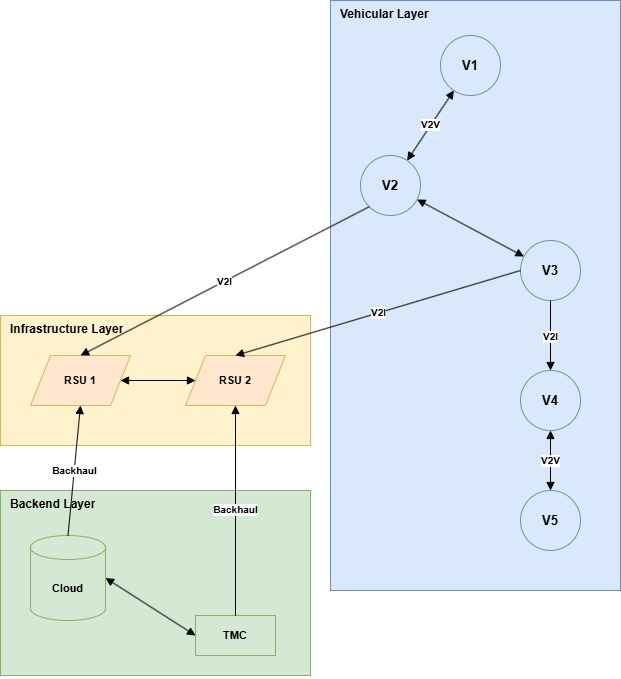
\includegraphics[width=0.5\textwidth]{figures/fig1.jpg}
	\caption{VANET architecture illustrating direct V2V communication links, V2I connectivity through roadside unit gateways, and backend integration with internet services and traffic management control systems. Adapted from \cite{karagiannis2011vehicular}.}
	\label{fig:vanet_architecture}
\end{figure}

\subsection{Performance Metrics and Evaluation Frameworks}

Evaluation of routing protocols for vehicular applications needs a multidimensional performance approach due to conflicting goals in the design of routing protocols for vehicular networks. No single metric can be used to fully describe a protocol's behavior, and those that try to optimize one dimension usually worsen other dimensions \cite{hartenstein2008tutorial}.

The Packet Delivery Ratio (PDR) is used to determine the ratio of sent packets that reach their destination nodes. The reason why the PDR is the most frequently quoted measure for evaluating VANET protocols is that it reflects what VANET protocols are supposed to do. But the PDR by itself is not a sufficient measure because one protocol may have good delivery rates while taking too long to deliver them, or low overheads but poor deliveries when there are few vehicles. This means that the PDR should always be considered along with the context in which it is evaluated.

Latency of end-to-end communication, defined as the total delay between packet transmission from the origin node and its successful delivery at the destination node, is the key limiting factor that restricts the range of possible solutions for mission-critical applications. There is a reason why 100 ms is the critical threshold for this type of communication—beyond this level, the efficiency of delivering safety-related messages drastically decreases. A forward collision warning received by a car after 200 ms delay since the trigger of the warning when driving at 100 km/h means that the vehicle has travelled another 5.5 meters by then. The physical laws impose limits on latency time, and any routing algorithm unable to function effectively under these conditions cannot be used for the given task irrespective of its performance rate \cite{li2007routing}.

The overhead caused by routing, which is defined as the percentage of the available channel capacity used by control information instead of actual data, is what makes the difference between scalable and non-scalable networks. A protocol using beaconing incurs control overhead that scales linearly with the number of nodes; hence, in a densely populated urban environment, the overhead caused by thousands of vehicles beaconsing can reach saturation without transmitting any single warning message.

\subsection{Simulation Methodologies and Their Limitations}

However, the vast majority of experiments regarding routing protocols in VANETs have been performed using simulations, and the accuracy of those simulations is the most crucial determinant of how well any findings can be extrapolated from the lab to real-life situations \cite{sommer2008progressing}.
The early VANET simulations relied on mobility models borrowed from MANET studies, namely random waypoint mobility models. Such methodology was disastrous for the validity of performance results reported based on such simulation studies. Indeed, the random waypoint mobility model does not mimic any of the properties that distinguish vehicular communication networks. Namely, constrained mobility is substituted by an unconstrained two-dimensional random walk; no speed correlation due to signal presence and no vehicle clustering near bottlenecks; and finally, no bimodal distribution for vehicles' spatial locations, which is typical of actual city traffic.

The appropriate approach to simulation should involve the use of microscopic traffic simulation by means of software like SUMO (Simulation of Urban MObility) to simulate car following behavior, lane changing, intersections and synchronization of traffic lights as well as network simulation by OMNeT++ using Veins or NS-3 with TraCI \cite{nzouonta2009vanet}. Such simulations accurately reflect the correlated movements, clustering at intersections and density dynamics observed in actual vehicular traffic. If the road geometry is not modeled in a simulation, the output generated by it cannot be used as proof of the effectiveness of any vehicular routing protocol.

Road topology data obtained from various sources including OpenStreetMap serves as input to the mobility simulation tool and the routing algorithm. It is worth noting that the technical world has slowly but surely adopted this method of simulation testing, and research papers that use this method yield more believable results than papers using simpler mobility assumptions.


%=================================================================
\section{Core Concepts and Approaches}
%=================================================================

Four main categories of routing protocols have been identified in the VANETs literature. Each of these categories rests on its own set of assumptions regarding network topology, infrastructure availability, and computation capabilities. The key challenge is to establish the range of applicability for each category and its limitations \cite{li2007routing}.

\subsection{Topology-Based Routing Protocols}

The topology-based routing protocols keep a representation of the network topology and determine their forwarding paths using that information. Topology-based routing protocols can be further classified into two sub-classes depending on whether the route is computed before or after sending requests for transferring data.

Proactive protocols such as the DSDV protocol and OLSR protocol keep the routing table of all destinations up-to-date at all times and proactively. Once there is a need to send information to any destination, the routing table can give us the route to send the message right away without wasting time on discovery. This is the greatest feature that proactive protocols have to offer. However, the greatest disadvantage of using proactive protocols is the continuous maintenance overhead incurred due to keeping the routing table up-to-date despite the changes in network topology. With respect to vehicular networks in which network topology changes because of the high-speed movement of vehicles, the maintenance overhead constitutes the greatest channel load. Even though OLSR protocol partly resolves this issue by defining Multipoint Relays to reduce the extent of flooding, the inherent scalability problem remains the same: as vehicular density increases, the network topology changes faster and more frequently \cite{perkins1994dsdv}.

The reactive family of protocols, including the widely used Ad hoc On-Demand Distance Vector (AODV) protocol and the Dynamic Source Routing (DSR) protocol, takes the completely opposite strategy of initiating route discovery when a data packet transmission is required \cite{perkins1999aodv}. Upon a requirement for a route to the destination by the source, an RREQ flood takes place across the network. The biggest drawback of the reactive family of protocols under vehicular conditions is that an RREQ flood overwhelms the channel before any data is sent. Also, due to fast change in topology, the route discovered becomes outdated before data packets can be sent over \cite{johnson1996dsr}. The threshold beyond which reactive protocols perform poorly is around 40-50 vehicles per kilometer.

\subsection{Geographic and Position-Based Routing Protocols}

Geographic-based protocols mark the largest innovation with respect to classical approaches in wireless network routing and have become the leading technique in urban vehicular scenarios \cite{mauve2001survey}. The core idea is that within a vehicular network, the position of a target node may be known either by means of a beacon exchange or vehicle localization system, and based on this alone, local routing optimization can be achieved.

Under the greedy forwarding approach, the choice of the next hop from each intermediate node occurs by choosing the neighboring node that is closest to the destination, resulting in a local greedy choice that eventually leads to the destination without having to maintain any state at any point in the route. Such a choice needs just three parameters: the position of the forwarding node, the position of the destination node, and the positions of neighbors. There is no discovery of a route prior to transmission, meaning there is zero discovery delay before starting the transmission process.

Greedy Perimeter Stateless Routing (GPSR), on the other hand, enhanced the simple concept of greedy routing through the introduction of perimeter routing for addressing the problem of void areas, where there is no neighbor which is geometrically nearer to the destination than the current node \cite{karp2000gpsr}. However, in an open environment like the rural highway network, the right-hand rule of GPSR can effectively bypass void areas, whereas this approach is bound to fail consistently in road networks.

The road-aware geographic variants overcome this problem by embedding the digital maps within the packet forwarding decisions themselves \cite{nzouonta2009vanet}. Instead of forwarding packets based on their geographical location to reach the destination, the packet forwards along road junctions in the path towards the destination. Performance tests have found that the road-aware protocols provide performance advantages of about 30-40 percent improvement in terms of packet delivery rate when compared to the map-oblivious alternatives.

\subsection{Broadcast and Geocast Protocols for Safety Applications}

The safety-related vehicular applications are always disseminated-based rather than unicast-based. The hazardous information, pre-emption messages for emergency vehicles, phase information for traffic signals, and road condition information need to be sent to all the vehicles present in the particular geographic area in a fixed duration of time irrespective of the set of vehicles that happen to be in the particular geographic region at the point of time when the message is sent \cite{vegni2015survey}.

The main problem that needs addressing from the viewpoint of vehicular communications is the issue of broadcast storms. As the original transmission of a safety message is received by numerous vehicles at once, all these vehicles will need to make the decision about whether they should retransmit the message themselves. The retransmission, if undertaken by all vehicles simultaneously, leads to a collision cascade, leaving no channel capacity for successful retransmission. There exist three kinds of rebroadcast suppression techniques, which have been proposed and studied so far. First, the distance-proportional rebroadcasting is a technique whereby the timing for rebroadcast is defined in such a way as to be inversely proportional to the distance from the rebroadcaster to the original broadcaster \cite{dressler2018not}. Second, probabilistic rebroadcasting defines the rebroadcasting probability of each candidate relay as inversely proportional to their own local neighbours. Third, network coding allows to algebraically combine several packets and transmit them through a rebroadcast.

It is equally critical for geocast zone delineation to have geographical bounds in terms of efficiency and safety considerations. Effective geographical delineation and filtering of the zones prevent safety messages from affecting their target geographic area only and not reducing the bandwidth of the distant network regions.

\subsection{Learning-Based and Adaptive Routing Protocols}

The latest and most technologically advanced advancement in vehicle routing involves the use of machine learning, and particularly reinforcement learning (RL), for vehicle routing decisions \cite{wang2020deep}. In the RL framework, routing is considered a problem of decision making under uncertainty, where an intelligent agent makes observations regarding the present state of the network, takes actions by choosing a route, and observes the result of its actions in terms of delivery success or failure.

Deep reinforcement learning, where the policy is represented by a neural network taking input from observations of high-dimensional states, generalizes this methodology to deal with the high-dimensional states encountered in vehicular networks \cite{mnih2015human}. Vehicle trajectories, quality-of-channel metrics, queue lengths, traffic density measurements, and historical delivery performance can all serve as input for the policy neural network, allowing for decisions made based on combinations of conditions not feasible using pre-programmed rules. Routing algorithms employing deep reinforcement learning techniques have been able to achieve near-optimal delivery rates in simulation experiments under varying vehicle densities.

There are two particular issues that prevent the practical application of RL-based routing from being shifted from simulation to real-world implementation. The issue of simulation to reality transfer relates to the incapability of policies developed using simulation to adapt to the dynamic nature of real-world traffic \cite{wang2020deep}. This problem can be solved via federated learning, a method for collaborative learning in real fleets of cars that does not necessitate centralized sharing of the trajectory and communication data among vehicles \cite{silva2022federated}. Each car learns and updates its routing policy locally and only shares gradient information with a centralized entity that uses it to learn an improved routing policy.

Figure~\ref{fig:taxonomy} presents the taxonomic classification of vehicular routing protocols across the four principal families identified in this analysis.

\begin{figure}[h]
	\centering
	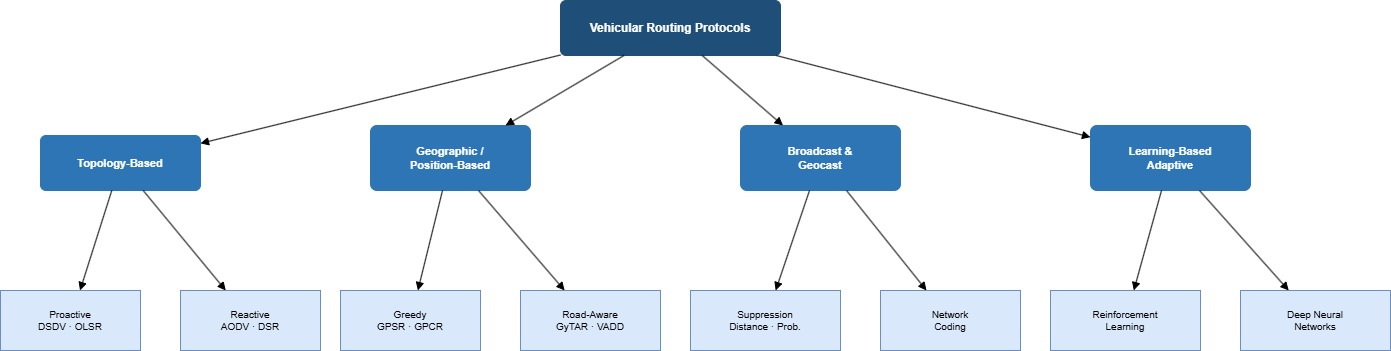
\includegraphics[width=0.75\textwidth]{figures/fig2.jpg}
	\caption{Taxonomic classification of vehicular routing protocols across the four principal families---topology-based, geographic, broadcast and geocast, and learning-based adaptive---with representative protocol instances for each category. Adapted from \cite{li2007routing,boukerche2011routing}.}
	\label{fig:taxonomy}
\end{figure}


%=================================================================
\section{Comparative Discussion}
%=================================================================

Not a single routing protocol outperforms the others in terms of performance under all deployment scenarios, types of applications, and performance attributes. This comparison study examines the protocols under various deployment scenarios, such as the variations in vehicular densities, urban structure, and multiple performance attributes including latency, overhead, and reliability \cite{boukerche2011routing}.

\subsection{Performance Variability Under Vehicular Density Conditions}

However, the most significant performance metric for the adoption of any protocol suite in an urban setting is its reaction to the variations in vehicular density, since a typical urban vehicular network will have to pass through all densities between sparse and hyper-dense over the course of a day \cite{li2007routing}.

The performance properties of reactive topology-based routing protocols are such that their quality of service degrades super-linearly above the threshold of connectivity at which point RREQ floods become self-interfering in nature. Below around 40 vehicles per kilometre, AODV can deliver messages satisfactorily in a fairly simple topology. Beyond this point, however, the RREQ floods caused by a single discovery operation spread to hundreds of nodes at once, each of which rebroadcasts the same message multiple times and interferes not only with other rebroadcasts but also with message transmissions.

The geographic protocol scales well with density since its routing decisions are completely local in nature. There is no need for global state to be maintained irrespective of the number of nodes, and routing decision computation is also computationally easy. Dense environments see good performance, with delivery rates being above 90% in simulation-based experiments using real mobile node models \cite{karp2000gpsr}. Sparse environments see expected degradation in performance when using the store and carry feature.

Learning protocols have the maximum flexibility to adjust their density profiles since the RL algorithm can learn various forwarding policies for each density scenario through learning as opposed to explicit coding \cite{wang2020deep}. Delivery ratios in simulations match optimal values for all density scenarios. The challenge arises due to the computation time involved; the inference of a deep neural network on embedded vehicle equipment takes place within milliseconds.

\subsection{Influence of Urban Road Structure on Protocol Performance}

Urban road networks have a wide variety of geometric designs depending on the city in question and the era when the city was developing, and their differences can affect the routing process.

The best case scenario for geographical forwarding is in North America’s grid cities, whose road network has a well-established structure consisting of regularly spaced rectangular blocks and intersection points occurring every four points. If we use the Manhattan grid, then the Euclidean distance of the destination is an acceptable estimate of the actual road network distance between two points, and map-oblivious forwarding algorithms have decent performance characteristics.

City centers in Europe and organically evolved cities pose a completely different problem altogether. The random nature of roads creates road networks in which the road distance between two places that are very close to each other may be up to three or four times the Euclidean distance, in which there are many roads that do not connect to any other, and in which Euclidean geometry is a poor indicator of connectivity. In such a situation, protocols that ignore maps perform poorly by a factor equal to the difference between Euclidean distance and road distance \cite{nzouonta2009vanet}.

The density of the RSU deployment will completely redefine the routing challenge irrespective of the nature of roads. High-density RSU regions will fragment long-distance hops involving multiple vehicles through vehicular relaying into one-hop vehicle-to-infrastructure communications. At this juncture, the routing challenge is reduced to choosing an RSU and routing from the RSU to the destination \cite{lequerica2010improvement}.

\subsection{Latency, Overhead, and Reliability Trade-offs Across Protocol Families}

The connection between latency, routing overhead, and reliability does not constitute a group of separate performance metrics---instead, they make up a restricted performance trade-off space, where an increase in one factor usually entails a decrease in another one \cite{li2007routing}. It is necessary to understand the particular nature of trade-offs for each protocol category.

The reactive topology-based protocol scheme has a distinct pattern wherein overheads remain very low in idle times but become extremely high when the discovery procedure takes place before every new data stream. The lag due to this high overhead is not suitable for use in safety-critical application since the overheads introduced will last a number of seconds. Reactive topology-based protocols will be able to work in low to moderate-density situations since their overheads depend on the time scale of seconds. The proactive topology-based protocols have an inverse pattern.

Geographic routing protocols have the best latency-overhead trade-off out of all the existing protocol categories. Since there is no need for any discovery stage, forwarding starts right away as soon as a packet is produced. The localized forwarding decision ensures that overhead is determined only by the rate of beacon transmission and the size of the zone, independent of the total size of the network \cite{mauve2001survey}.

Broadcast and geocast algorithms take a distinct place in the trade-off area. These techniques provide exceptionally reliable communication with exceptionally small delays in the respective geographic areas, but they come at an extremely high cost in terms of the overhead of the channel in the respective geographic regions. This technique is best suited for safety-critical communication scenarios.
Table~\ref{tab:comparison} presents a structured comparative analysis of the four protocol families across the key performance dimensions.

% ---------------------------------------------------------------
%  TABLE 2 — Comparative analysis table (fixed)
% ---------------------------------------------------------------
\begingroup
\renewcommand{\arraystretch}{1.5}
\begin{table}[H]
	\centering
	\caption{Comparative analysis of vehicular routing protocol families across key
	         performance dimensions under urban deployment conditions with mixed
	         vehicular density.
	         Sources: \cite{li2007routing,boukerche2011routing,karp2000gpsr,wang2020deep}.}
	\label{tab:comparison}
	\begin{tabular}{|>{\hyphenpenalty=10000\exhyphenpenalty=10000\raggedright\arraybackslash}p{3.2cm}|>{\hyphenpenalty=10000\exhyphenpenalty=10000\raggedright\arraybackslash}p{1.6cm}|>{\hyphenpenalty=10000\exhyphenpenalty=10000\raggedright\arraybackslash}p{1.8cm}|>{\hyphenpenalty=10000\exhyphenpenalty=10000\raggedright\arraybackslash}p{2.8cm}|>{\raggedright\arraybackslash}p{4.2cm}|}
		\hline
		\textbf{Protocol Family} &
		\textbf{Latency} &
		\textbf{Overhead} &
		\textbf{Delivery Reliability} &
		\textbf{Deployment Assessment} \\
		\hline
		Proactive Topology-Based
		    & Low & High & Moderate &
		    Legacy approach; suitable only for stable RSU backhaul links and fixed
		    infrastructure corridors. \\[4pt]
		\hline
		Reactive Topology-Based
		    & High & Low--Mod. & Moderate &
		    Obsolete above 50 vehicles/km; incompatible with safety-critical latency
		    requirements. \\[4pt]
		\hline
		Geographic / Position-Based
		    & Low & Low--Mod. & High (dense); Moderate (sparse) &
		    Current best-practice default. Road-aware variants are mandatory in
		    organic urban topologies. \\[4pt]
		\hline
		Broadcast / Geocast
		    & Very Low & High & Very High &
		    Reserved for safety-critical dissemination. Storm suppression is
		    non-negotiable. \\[4pt]
		\hline
		Learning-Based Adaptive
		    & Low--Mod. & Moderate & High &
		    Near-future standard. Sim-to-real transfer gap remains the key
		    deployment barrier. \\[4pt]
		\hline
	\end{tabular}
\end{table}
\endgroup


%=================================================================
\section{Practical Insights and Use Cases}
%=================================================================

Indeed, the transition of performance testing results in simulations to real-world applications constitutes one of the most challenging tasks for the field of intelligent vehicular routing protocols. In this regard, this chapter will focus on four different application scenarios, which altogether cover the entire scope of application areas for intelligent vehicular routing protocols.

\subsection{Traffic Signal Optimisation and Green Wave Corridor Management}

Traffic signal optimisation use case scenario is considered to be the most developed and widely implemented use case scenario for vehicular communication and routing. The basic idea of traffic signal optimisation is quite clear: in case when the approaching vehicles can successfully communicate with the traffic signal controller their estimated time of arrival, the controller will be able to set up optimal signal phases duration and minimize the total stop time of the conflicting traffic flows.

Routing is a well-defined and straightforward problem for this application: reliable and low-latency unicast delivery from the approaching vehicle to the RSU collocated with the intersection traffic light controller. This requires routing to a stationary infrastructure node at a known geographical location, so geographic routing toward the intersection RSU becomes an obvious choice for the problem. The performance requirement is modest compared to other applications in VANETs---it is adequate to achieve delivery ratios exceeding 95 percent and latencies less than 500 milliseconds.

The green wave corridor approach builds on the idea of traffic lights optimisation at each individual intersection point to manage the coordinated operation of traffic signals over a series of intersections along an important arterial road. The system of speed advisory messages should be able to inform the vehicle drivers at least 500 meters or more in advance of the upcoming green wave intersection so that they can reduce their speed accordingly \cite{karagiannis2011vehicular}. European implementations of the technology have shown steady reductions of 20 to 35 percent in travel times.

\subsection{Emergency Vehicle Pre-emption and Priority Routing}

Pre-emption for emergency vehicles is the safety-critical scenario, which demonstrates the importance of the life-and-death implications involved in vehicular routing protocols. In case an emergency vehicle approaches, it sends out information about its identity, its path, and its projected time of arriving at future intersections; as such, the system will prolong green light intervals or initiate a new phase in order to make room for the emergency vehicle \cite{hartenstein2008tutorial}.

However, the routing problem is much more complicated than the previous example of cooperative signal optimisation, where the broadcast needs to be sent to several recipients at once: the intersections up ahead of the car, civilian cars on the road, and traffic management systems. Ineffectual propagation of pre-emption messages down the emergency car’s intended route will cause signal disruptions in places that do not have any use for pre-emption and will disrupt traffic flow to such an extent that it may even hinder the emergency vehicle from reaching its destination \cite{vegni2015survey}.

\subsection{Freight and Logistics Network Optimisation}

The field of freight and logistics offers a unique perspective on the routing application paradigm due to its diverse needs in terms of latency, size of the vehicle, and route predictability compared to passenger vehicles \cite{akyildiz2005wireless}. There are two main instances where the routing needs vary depending on the scenario.
For long haulage truck freight optimization, real-time traffic density information from the vehicle network will be used to allow diversion of trucks away from busy routes until the congestion is alleviated. For the latency requirement of this application, seconds to minutes is much more suitable than milliseconds since the effect of diverting the traffic will take a considerable period of time. In this case, the reliability factor outweighs the latency factor, and geographic unicast to RSU gateways with cellular backhaul connections to the fleet management system will be enough. It has been shown by simulations and real world experiments that the average reduction in delivery time variance is between 15% to 20% \cite{lequerica2010improvement}.

The coordination of urban last-mile delivery encompasses the simultaneous coordination of several delivery trucks within the same urban regions. The integration of fleet management allows for the scheduling of trucks to bypass busy loading docks, share information on available parking spots to minimize search time for delivery spots, and synchronize delivery windows across several trucks to minimize overall parking requirements \cite{akyildiz2005wireless}.

\subsection{Intelligent Highway Management and Platooning Support}

The ability to manage highways cooperatively using vehicle-to-vehicle communications allows several functionalities that cannot be provided without communications among the vehicles, such as lane coordination, on-ramp metering support, and high-density platooning \cite{hartenstein2008tutorial}. Highways may be easier environments for the routing protocol design in some aspects compared to urban environments, where the road structure is simpler to model due to its one-dimensional nature and vehicular density is more predictable, while the communication distance does not depend on building obstruction problems. However, highways are also harder environments because of the higher speeds of all entities and shorter lifetimes of their links.

Platooning, or cooperative group formation and management, poses the greatest technical challenge to highway routing. In a platoon, the network structure remains constant, forming a linear chain throughout its lifetime; this makes it possible to do routing optimizations for high throughput and low latency in communicating down the chain. The need for inter-platoon coordination goes beyond the capabilities of DSRC-type communications and needs the use of cellular V2X technology, which, in turn, calls for routing protocol support for both short-range and long-range infrastructural routes.


%=================================================================
\section{Challenges and Open Issues}
%=================================================================

The difference between the performance achieved by the routing protocols through simulations and the performance possible on large-scale implementations in the production environment can be addressed by solving a series of technical problems, which have been identified in the literature but not solved \cite{zheng2015heterogeneous}. These problems will be outlined in this section, with enough technical detail to distinguish them from mere optimization problems.

Position information integrity is perhaps the most basic challenge to the functioning of position-based routing. The geographical nature of such forwarding algorithms means that they require reliable information about position, and a malicious node can easily disrupt forwarding throughout a large part of the network through broadcasting fake positional information \cite{zheng2015heterogeneous}. Similarly, a Sybil attack in which a malicious party generates several fake nodes with unique positions can lead to forwarding through non-existent forwarding routes that eventually end up at a black hole. Certificate-based cryptographic authentication offers a sound countermeasure for this challenge, provided there is an existing vehicular public key infrastructure; however, the use of such certification introduces processing complexity per forwarding decision and reliance on a distributed certificate authority system, both of which do not exist at present in any vehicle-to-vehicle networking technology.

The gap between simulations and the real world poses an entirely new challenge for learning-based algorithms compared to deterministic routing protocols. In case a deep RL routing algorithm has been trained using simulations, the algorithm’s policy will be tuned towards the particular statistical properties of the simulated environment, such that when some statistical properties exist in the simulator and do not exist in the real world, then this will make the policy fail when used in the real world \cite{mnih2015human}. Federated learning using a fleet of vehicles appears to be the only realistic solution, although federated learning poses several challenges of its own \cite{silva2022federated}.

Fleet heterogeneity is an operational issue for which there does not seem to be a solution in the current research. The type of vehicles expected to travel within any given urban area in the coming two to three decades will include vehicles without any capability of wireless communication, vehicles that are capable of DSRC alone, vehicles that have both DSRC and C-V2X capabilities, partly autonomous vehicles with enhanced sensory ability but inconsistent communication ability, and completely autonomous vehicles with all the sensors and V2X capabilities.Routing algorithms that assume fleet homogeneity will be ineffective once put into use in such a scenario \cite{li2007routing}.

The fragmentation of regulation at the national and regional levels can be seen as a problem of coordination that may be harder to address than any of the technical problems. There are differences in frequency spectrum allocation among vehicular communication in the United States, the European Union, Japan, and China. There is no agreement on the certification of vehicular communication devices. The legal framework for liability for the autonomous decision-making capability of vehicular communication is still in its infancy. While IEEE, ETSI, and 3GPP have achieved considerable success in technical matters such as standardisation of protocols and interoperability, the translation of these technical issues into regulatory problems lags behind.


%=================================================================
\section{Future Directions}
%=================================================================

The future trajectory of routing technology for vehicles is likely to be determined by a number of concurrent trends within wireless networks, self-driving cars, urban sensing, and artificial intelligence, all of which have entered their early stages of implementation \cite{zheng2015heterogeneous}. The following sections highlight each trend and its implications for route planning protocols.

Fifth generation and even more so the future sixth generation of cellular technology built into the vehicle communications chain is clearly the most structurally revolutionary change in the short term. 5G New Radio V2X, which is already being standardized by 3GPP, has the ultra-low latency, extreme device density capability, and network slicing that would make safety critical communication possible using cellular networks instead of DSRC. If 5G technology were widely adopted in urban vehicular scenarios, the relay multi-hop routing problem that has driven VANET research for almost twenty years would be made moot. 6G cellular communications, capable of sub-100 microsecond latency in vehicular settings, would completely end the VANET routing problem in about a decade.

Incorporating smart city infrastructure into an integrated system makes it possible for a holistic approach to urban mobility management where routing decisions can be viewed as a part of broader optimisations across the entire urban transportation network \cite{naumov2007connectivity}. Routing decisions regarding individual sessions of vehicle communications can be synchronized with other elements of the urban transportation system such as signals at intersections, public transport timetables, shared mobility systems, parking availability and pedestrian movement in order to yield results for the transportation system which would be impossible to achieve with a vehicle-based route decision alone.

CAV platoon networks present an interesting case in terms of communication topology, which is fundamentally different from the conventional vehicle routing problem and requires dedicated protocols \cite{hartenstein2008tutorial}. In terms of a stable platoon network, the network topology is static and linear, where the participating vehicles and their communication capabilities are known beforehand, allowing for dedicated optimization of the routing protocol based on the properties of the linear topology. However, inter-platoon communication necessitates long-range cooperation beyond the limits of direct communication links, thus calling for cellular V2X communication with backend intervention.

The combination of edge computing and RSUs appears to be a promising strategy for addressing the computational feasibility issues that are currently hindering the implementation of learning-based routing \cite{karagiannis2011vehicular}. The transfer of the computationally intensive process of routing optimisation from embedded vehicle processors to co-located edge servers with far more powerful computational capabilities removes the embedded inference latency issue but adds an additional round-trip latency to the edge server. The use of semantic communication involves a paradigm shift towards identifying what should be the content of vehicular communication protocols \cite{dressler2018not}. Semantic communication would only communicate information relevant to the task at hand, resulting in one order of magnitude less overhead in communications.


%=================================================================
\section{Conclusion}
%=================================================================

Intelligent routing protocols for smart transportation networks have advanced significantly from the early adoption of MANET routing protocols to the present state where it represents an engineering science based on the particularities of vehicle-based networks. In this paper, we have reviewed intelligent transport networks from its conception and theoretical framework to the contemporary state-of-the-art and into the potential research directions that exist in the future, paying constant consideration to the mismatch between performance in simulation versus actual application.

The first key insight from comparative study is that no family of protocols performs uniformly better across all deployment scenarios. The use of topology-based protocols is valid only in stable RSU-based network segments, if the cost of overhead and delay involved can be tolerated. Road aware geo-routing is the current best practice protocol to deploy as default choice for urban vehicular networks, which can provide consistently low delay and scalability in bimodal traffic density conditions. Broadcast and geocast protocols are the inevitable solution for applications in safety critical information dissemination, since storm filtering mechanisms must be provided. Learning based adaptive protocols offer the most promising direction towards future deployments, in which adaptability of the protocol to conditions beyond those envisioned by any preconceived rulesets can be offered, but hindered by simulator to reality gap and inference delay problems.

The problems identified in this paper—falsified positioning and Sybil attacks targeting geographic routing, heterogeneity in fleet composition, regulatory fragmentation, and federated learning convergence—are not mere optimizations to achieve. They are the actual gap between what research papers say and the implementation of technology capable of delivering safety benefits and reducing congestion in urban environments. Addressing these problems would require long-term cooperation among experts in wireless communications, transportation engineering, artificial intelligence, cybersecurity, and policy makers who can turn technological developments into regulations for widespread adoption.

The external environment in which this evolution needs to take place includes the proliferation of 5G and future 6G cellular technologies, the expansion of connected and partially autonomous cars, advanced smart city sensing and management technologies, and fast-moving advances in machine learning algorithms and hardware. All of these trends together provide the context in which intelligent routing technology for our vehicles must develop and mature. The cities that will successfully implement intelligent routing in their vehicular transportation networks can expect to see many clear gains in terms of efficiency, energy usage, safety results, and overall urban quality of life. The underlying technology is ready for this leap; all that is left is the application and integration expertise to realize it.


\bibliographystyle{plain}
\bibliography{references}

\end{document}